\documentclass[twocolumn,prd,superscriptaddress,nofootinbib]{revtex4-2}

\usepackage{amsmath,amssymb}
\usepackage{graphicx}
\usepackage[hidelinks]{hyperref}
\widowpenalty=10000
\clubpenalty=10000

\newcommand{\SolarA}{0.0087502019}
\newcommand{\SolarAlpha}{0.1244971139}
\newcommand{\DimensionFloor}{2.973749394}
\newcommand{\GRPeakMass}{2.0497850}
\newcommand{\GRRadius}{11.685866}
\newcommand{\GRLambda}{298.0203}
\newcommand{\GRLove}{0.07746217}
\newcommand{\LambdaOne}{286.07414}
\newcommand{\TidalShiftOne}{-4.00852}
\newcommand{\RadiusShiftOne}{-0.42506}
\newcommand{\LoveShiftOne}{-1.94212}
\newcommand{\RadiusOnlyOne}{-2.10732}
\newcommand{\CrossTermOne}{0.04093}
\newcommand{\MismatchOne}{1.29793}
\newcommand{\BinaryOne}{345.43908}
\newcommand{\LambdaTwo}{286.72902}
\newcommand{\TidalShiftTwo}{-3.78878}
\newcommand{\RadiusShiftTwo}{-0.40225}
\newcommand{\LoveShiftTwo}{-1.83018}
\newcommand{\RadiusOnlyTwo}{-1.99511}
\newcommand{\CrossTermTwo}{0.03651}
\newcommand{\MismatchTwo}{1.31654}
\newcommand{\BinaryTwo}{346.16640}
\newcommand{\BinaryGR}{359.54855}


\begin{document}
\raggedbottom

\title{Radial Dimensionality Theory III: Neutron Star Structure under Solar-Constrained Density-Dependent Dimensionality}
\author{Christopher K. Merrill}
\affiliation{Independent Researcher}

\author{Claude (Anthropic)}
\affiliation{Large Language Model, Computational Collaboration}

\author{Astra (Open AI)}
\affiliation{Large Language Model, Computational Collaboration}

\date{Consistency revision: November 12, 2026}

\begin{abstract}
We propagate a conditional solar model/proxy region through two
phenomenological neutron-star prescriptions using the full density-dependent
law of Radial Dimensionality Theory. The calculation uses the documented
CompOSE RG(SLy4) equation of state, corrected central seeds and separately
checked numerical formulations. A scan of 1,980 parameter rows and 24 local
refinements samples 70 density exponents and physical reference lengths of
5, 10 and 20 km. At 10 km the largest sampled Embedding~1 deficits are
0.711680\% in the largest mass found within the EOS domain and 0.425782\%
in radius at $1.4M_\odot$. The modified sequences at these extrema reach
the EOS pressure boundary without a bracketed turnover; the mass result
is therefore not an established maximum-mass shift. All 396 five-point
amplitude traces are monotonic on the tested points. These results are
finite samples, not continuum or EOS-independent bounds. Paper~IV computes
conditional tides at a common, explicitly identified solar-amplitude-peak
point, obtaining $\Delta\Lambda_{1.4}/\Lambda_{1.4}=\TidalShiftOne\%$.
Its prescribed Schwarzschild extraction retains an unresolved boundary
matching assumption. All producing scripts and numerical evidence are
retained in the accompanying GitHub repository.
\end{abstract}
\maketitle

\section*{Version note: v9}
This version retains the published title. It uses the full density law and corrected central seeds, comparing two specified hydrostatic prescriptions for one equation of state over a sampled parameter domain. The reported mass extrema occur at the equation-of-state domain boundary and do not establish shifts in the true maximum stable mass. The conditional tidal example is reconciled with Paper IV, with the finite cutoff and exterior-matching limitations explicit.


\section{Scope and solar input}
Neutron-star masses, radii and tidal responses depend on the dense-matter
EOS and the gravitational prescription \cite{Lattimer2016,Oertel2017}.
Here we quantify the response of two specified models, rather than fitting
a new EOS or inferring a unique gravitational completion.
Papers~I--II supply a shared density law and a conditional solar region
\cite{PaperI,PaperII,WorkingEvidence}:
\begin{align}
 d_{\rm eff}&=3+\delta, &
 \delta&=-3A\frac{x}{1+x},\\
 x&=(\rho_b/\rho_{\rm ref})^\alpha, &
 \rho_{\rm ref}&=150~{\rm g\,cm^{-3}}.
\end{align}
The law density is baryon rest-mass density $\rho_b$, not total energy
density divided by $c^2$. The reference density is a series convention.

We use Paper~I's source-precision diagonal proxy score and its nominal
$\Delta Q=2.71$ slice thresholds, denoted $A_{\rm lim}(\alpha)$.
This notation replaces the potentially misleading confidence-limit label
$A_{95}$: observational coverage has not been calibrated. The solar
polytropic response, chosen observational errors and helioseismic proxy
remain assumptions of the propagated region. The selected locally refined
solar-amplitude peak is
\begin{equation}
 (\alpha_\star,A_\star)=(\SolarAlpha,\SolarA).
 \label{eq:point}
\end{equation}
Its dimensional asymptote is $3-3A_\star=\DimensionFloor$, not a strict
universal floor $d_{\rm eff}>2.974$. Neither this point nor the sampled
region is a certified continuous-domain confidence envelope.

The solar-amplitude peak need not maximize a neutron-star response.
We distinguish Eq.~(\ref{eq:point}), used for the shared Paper~IV example,
from the NS extrema located by the finite sampling below. A specified
phenomenological model can be tested against data without outside
endorsement; numerical checks and explicit assumptions determine which
model that test addresses.

\section{Background prescriptions}
\subsection{Density sources and reference length}
The operator-motivated Newtonian equation is
\begin{equation}
 \frac{1}{r^2h}\frac{d}{dr}(r^2h a)=4\pi G\rho_b,
 \qquad h=(r/r_\star)^{\delta(\rho_b)}.
\end{equation}
The physical reference length $r_\star$ makes the variable-exponent
weight well defined. A change of units rescales $r$ and $r_\star$
together; changing the physical reference length changes the model.
The primary value is 10 km; 5 and 20 km are sensitivity choices.
This differs from Papers~I--II's Lane--Emden-scale prescription.

For the structure equations below, use geometrized units $G=c=1$,
with energy density $e$ and pressure $p$. The law above continues to use
the physical baryon density relative to its stated reference density.
Define ordinary energy mass $m$, ordinary baryon integral $B_0$, weighted
baryon integral $B_\delta$ and weighted energy integral $E_\delta$:
\begin{align}
 m'&=4\pi r^2 e,& B_0'&=4\pi r^2\rho_b,\\
 B_\delta'&=4\pi r^2h\rho_b,& E_\delta'&=4\pi r^2h e.
\end{align}
Here the baryon source is converted consistently to geometrized units;
its common normalization cancels in the field ratio. Set
\begin{equation}
 f=1-2m/r,\qquad q=B_\delta/(hB_0).
\end{equation}
Both prescriptions retain ordinary energy mass in $f$ and satisfy
\begin{equation}
 p'=-(e+p)g,\qquad g=\frac{D}{r^2 f},
\end{equation}
with
\begin{align}
 D_1&=q(m+4\pi r^3p),\label{eq:emb1}\\
 D_2&=E_\delta/h+4\pi r^3p.\label{eq:emb2}
\end{align}
These explicit equations remove ambiguity about pressure weighting in
Embedding~2. They reduce to the same GR system at $A=0$ and have checked
cold Newtonian limits. They are two conditional prescriptions, not a
unique covariant completion or an exhaustive theory-uncertainty model.
Hydrostatic balance specifies $\nu'=2g$ if an isotropic-fluid metric
interpretation is adopted; it does not supply all field equations.

\subsection{EOS and finite surface}
Only the 197-point CompOSE RG(SLy4) table is used for the current
parameter predictions \cite{CompOSE,WorkingEvidence}. Its source members,
indices, units and conversions were checked. Total energy density and
$\rho_b=m_u n_b$ are kept distinct. The separate Douchin--Haensel source
regression \cite{Douchin2001} checks 77 retained crust/core rows and the
historical energy-convention error; it is not a second EOS-family test.
APR predictions remain withdrawn.

The integration stays inside the documented EOS pressure range and ends
at $P_s=1.001P_{\min}$. No crust extension or high-density extrapolation
is invented. This defines a finite-pressure radius, not an exact
zero-pressure stellar surface. Changing the cutoff is a model-scope
sensitivity distinct from integration error. A maximum-mass assertion
requires a turnover bracketed within supported EOS data.

\section{Numerical calculation and controls}
The primary solver integrates five flux states in $t=\ln(P_c/P)$ with
DOP853. It uses corrected regular-center seeds at $r_0=100$ cm.
Writing $p=p_c-\beta r^2+\cdots$, the leading coefficients are
\begin{align}
 \beta_1&=2\pi(e_c+p_c)(e_c/3+p_c)\frac{3}{3+\delta_c},\\
 \beta_2&=2\pi(e_c+p_c)\left(\frac{e_c}{3+\delta_c}+p_c\right).
\end{align}
Weighted central integrals contain $1/(3+\delta_c)$, not $1/3$.
An independent radial-field integration checks the flux formulation.
Nonfinite states, failed termination and out-of-range EOS access are
errors; failed points are not silently omitted.

The main scan uses rtol $2\times10^{-9}$, atol $10^{-17}$ and maximum
log-pressure step .1. The shared GR baseline is tighter. Each parameter
row uses nine log-spaced central pressures from $5\times10^{34}$ to the
EOS maximum, plus four near-edge probes; local interior peaks are refined.
A separate bracketed root finds the radius at $1.4M_\odot$.

The original 66 solar slices consist of 65 exponents from .02 to .5 and
Eq.~(\ref{eq:point}). Five amplitude fractions (0, .25, .5, .75, 1), two
prescriptions and three reference lengths give 1,980 rows. The 396 null
rows reuse a checked GR baseline. Two local exponent-refinement rounds
recompute four solar endpoints and add 24 NS rows; endpoints are not
interpolated from the accepted contour.

The 38 selected controls include tighter integration/pressure grids,
central-start changes, PCHIP interpolation, an independent radial-field
solver and full-saturation diagnostics. Tightening changes fractional
mass/radius shifts by at most $7.06\times10^{-8}$/$2.24\times10^{-7}$;
the independent fixed-mass radius shifts agree within $4.29\times10^{-8}$.
PCHIP changes shifts by up to $1.10\times10^{-6}$/$2.38\times10^{-6}$.
These measured comparisons support the tested results, not a uniform
error bound over all parameters or an EOS uncertainty band.

\section{Results}
\subsection{EOS-domain mass and sampled extrema}
The checked GR domain peak is $\GRPeakMass M_\odot$, with a shallow
interior turnover; its $1.4M_\odot$ radius is approximately
$\GRRadius$ km. Define $M_{\rm dom}$ as the largest mass found by the
supported pressure-grid and local-refinement procedure. At all extrema
in Table~\ref{tab:extrema}, the modified sequence reaches the upper EOS
pressure edge. Its $M_{\rm dom}$ is not an established true maximum mass.

\begin{table}[t]
\caption{Most negative sampled shifts, in percent. Mass and radius
extrema are selected separately. The mass column is EOS-domain limited;
the table does not certify a continuum envelope.}
\label{tab:extrema}
\centering\small\setlength{\tabcolsep}{3pt}
\begin{tabular}{cccc}
\hline\hline
$r_\star$ (km) & Emb. & $\Delta M_{\rm dom}/M$ (\%) & $\Delta R_{1.4}/R$ (\%) \\
\hline
5 & 1 & -0.710099 & -0.420488 \\
5 & 2 & -0.570314 & -0.397669 \\
10 & 1 & -0.711680 & -0.425782 \\
10 & 2 & -0.571696 & -0.402947 \\
20 & 1 & -0.713264 & -0.431176 \\
20 & 2 & -0.573077 & -0.408294 \\
\hline\hline
\end{tabular}

\end{table}

\begin{figure*}[t]
\centering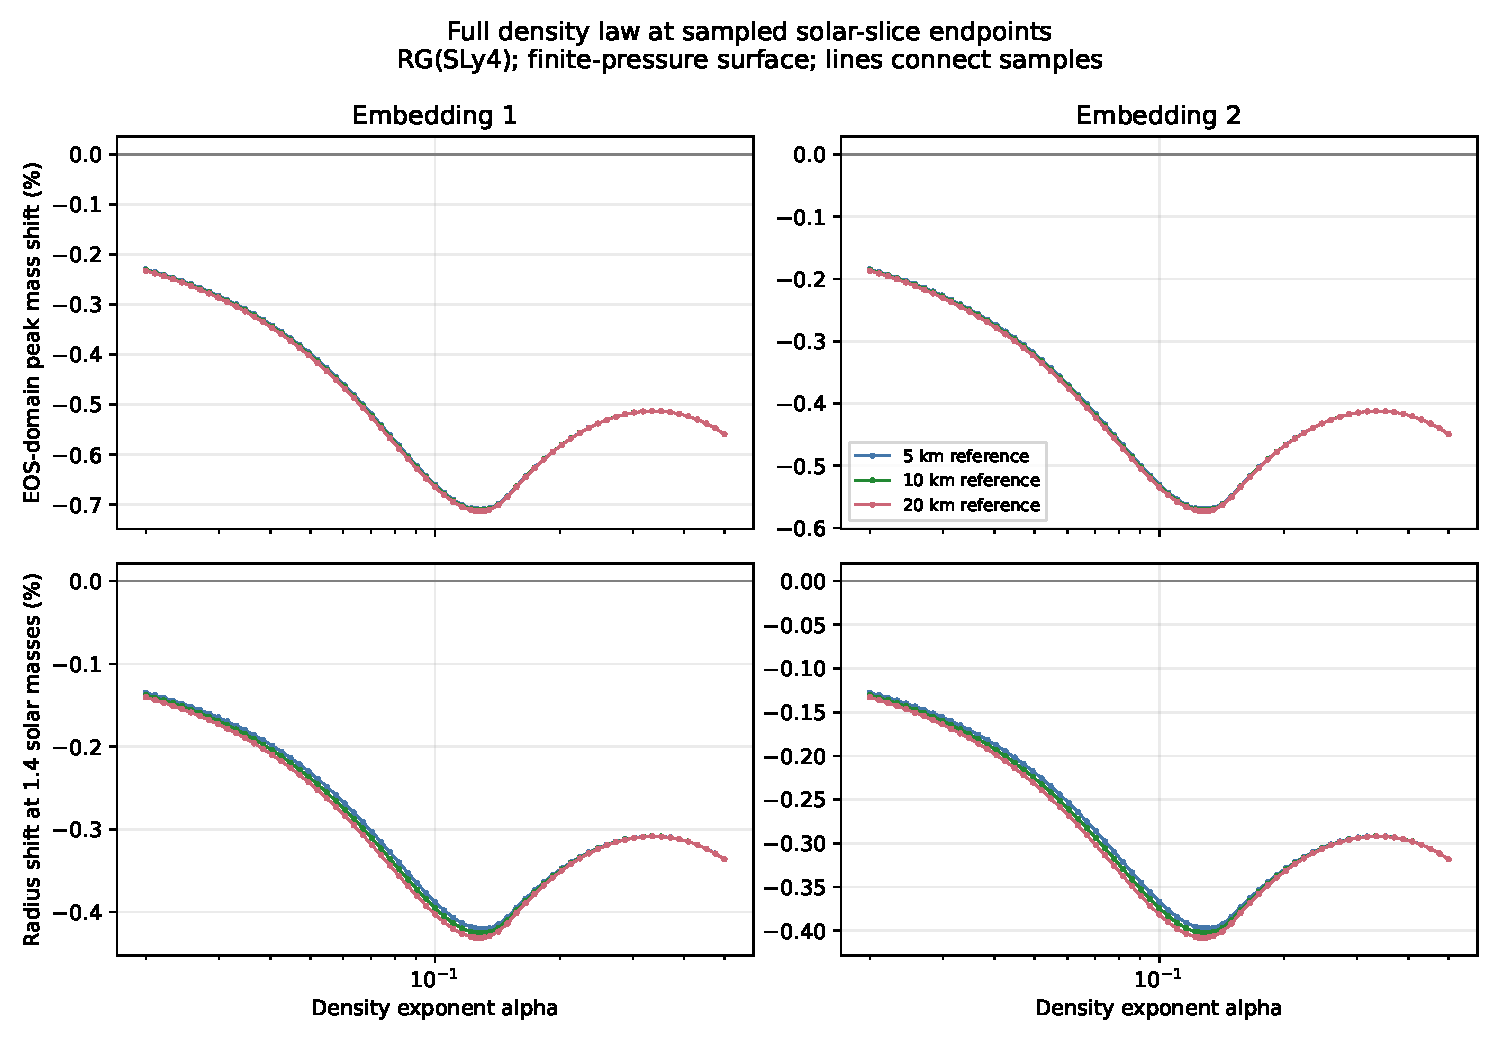
\includegraphics[width=.95\textwidth]{ns_parameter_dependence.pdf}
\caption{Full-law response at sampled solar-slice endpoints for both
prescriptions and three physical reference lengths. Connecting lines
are guides between samples, not confidence envelopes. Mass shifts refer
to the largest mass found within the EOS domain; they are not uniformly
interpretable as true maximum-mass shifts. The finite-pressure surface
and CompOSE RG(SLy4) EOS are common to all curves.}
\label{fig:parameters}
\end{figure*}

All sampled mass extrema occur at $\alpha=.1285920332$ and
$A=.008738820028$. Radius extrema occur at $\alpha=.1302191231$,
$.1285920332$ and $.1275558462$ for 5, 10 and 20 km, respectively.
All 396 five-point amplitude traces are nonincreasing in both shifts;
continuous monotonicity is not proved. Across matched nonzero-amplitude
samples, changing the reference length from 5 to 20 km produces spans
up to .00640431 percentage points in mass shift and .0161503 percentage
points in radius shift. The two-prescription spread does not exhaust
model uncertainty.

The full law matters at low exponent. Replacing it by constant
$\delta=-3A$ in six diagnostic cases changes the fractional mass and
radius shifts by up to .00126418 and .000773748, respectively, at
$\alpha=.02$. Uniform saturation over the allowed exponent range is
therefore not an adequate approximation for this calculation.

\subsection{Common point with Paper IV}
Table~\ref{tab:common} uses Eq.~(\ref{eq:point}) at 10 km, not the
NS extrema in Table~\ref{tab:extrema}. Both papers use identical
parameter records and the same EOS, source conventions and surface.
The table's radii and domain masses come from the background scan;
the tidal values come from the separately checked augmented integrations.
Their background radii agree within the prescribed $5\times10^{-7}$
fractional tolerance.

\begin{table}[t]
\caption{Shared solar-amplitude-peak example. $M_{\rm dom}$ is in solar
masses. The modified domain peaks reach the EOS boundary. Tides include
the additional prescriptions specified in Paper~IV.}
\label{tab:common}\centering\small
\begin{tabular}{cccc}
\hline\hline
Emb. & $M_{\rm dom}/M_\odot$ & $R_{1.4}$ (km) & $\Lambda_{1.4}$ \\
\hline
1 & 2.0352165 & 11.636192 & 286.0741 \\
2 & 2.0380823 & 11.638859 & 286.7290 \\
\hline\hline
\end{tabular}

\end{table}

Paper~IV obtains GR $\Lambda_{1.4}=\GRLambda$ and
$\Lambda_{1.4}=\LambdaOne$ (Embedding~1), a
$\TidalShiftOne\%$ change. Radius-only scaling is insufficient: the
exact radius contribution is $\RadiusOnlyOne\%$, while $k_2$ changes
$\LoveShiftOne\%$, with a positive multiplicative cross term.
Embedding~2 gives $\TidalShiftTwo\%$ under the same tidal prescription.
These are conditional samples, not sub-percent tides or global ceilings.

The tidal calculation uses a prescribed Schwarzschild exterior. The
computed interior does not yet satisfy smooth metric-gradient matching
to that exterior at the chosen surface; the mismatch is approximately
$\MismatchOne\%$ in the primary example. The tidal response depends on
this unresolved boundary prescription. That mismatch is not an estimated
percentage error in $\Lambda$.

\section{Interpretation and revision history}
The tested full-law samples reduce radii and domain-limited mass support
relative to their paired GR baselines. They neither resolve every soft-EOS
heavy-pulsar problem nor establish an EOS-independent sign law. A calibrated
observational exclusion or forecast requires an explicit data likelihood,
EOS treatment and the stated gravity/perturbation assumptions. Such a test
does not require outside endorsement of the phenomenological model.

Earlier force-multiplier results remain results of a different prescription,
not evidence that one sign is mandatory. The energy-density reconstruction
error, crust truncation and unsupported APR results from prior versions
remain withdrawn. The earlier approximately .71\%/.42\% examples are
replaced here by reproducible finite-domain sampling and explicit peak
classification. The old .12 versus .122 parameter-label discrepancy is
avoided by the common full-precision input record. Historical scripts,
failed/interrupted runs and released PDFs remain preserved.

The open physical questions are the EOS extension, a covariant completion,
and the perturbation/exterior matching problem. They must not be confused
with the numerical checks completed here. The paper's predictions are the
conditional outputs of the explicit equations and sampled inputs above.

\section*{Code and revision availability}
Producing scripts, inputs, saved results and numerical audit evidence are
publicly available in the \href{https://github.com/chrismerrill1974/solarcore_code/tree/main/reproduction}{shared RDT reproducibility archive}.
The accompanying source package, \nolinkurl{merrill2025_neutronstar_code}, includes the
manuscript, dependencies and resource-controlled reproduction commands.
Its \texttt{reproduction/CAPSULE.json} records file hashes;
\texttt{reproduce.py} verifies the package and rebuilds the paper from retained
scientific outputs. Full scientific runs are separate from this saved-result
reproduction. Historical scripts and results remain separately identified.

\section*{Acknowledgments}
Computational collaboration: Astra (Open AI) and Claude (Anthropic).
We thank the developers of NumPy, SciPy and Matplotlib, CompOSE, and the
authors of the source EOS tables.

\begin{thebibliography}{99}
\bibitem{Lattimer2016} 
J.~M.~Lattimer and M.~Prakash, 
``The equation of state of hot, dense matter and neutron stars,''
Phys. Rep. \textbf{621}, 127 (2016).

\bibitem{Oertel2017}
M.~Oertel, M.~Hempel, T.~Kl\"{a}hn, and S.~Typel,
``Equations of state for supernovae and compact stars,''
Rev. Mod. Phys. \textbf{89}, 015007 (2017).

\bibitem{PaperI} C.~K.~Merrill, Claude (Anthropic), and Astra (Open AI),
``Radial Dimensionality Theory I: Solar Neutrino and Helioseismic Constraints on Density-Dependent Spatial Dimensionality,''
revised version, November 12, 2026.

\bibitem{PaperII} C.~K.~Merrill, Claude (Anthropic), and Astra (Open AI),
``Radial Dimensionality Theory II: White Dwarf Structure under Solar-Constrained Density-Dependent Dimensionality,''
revised version, November 12, 2026.

\bibitem{WorkingEvidence}
C.~K.~Merrill, Claude (Anthropic), and Astra (Open AI),
RDT working consistency revision: source inputs, numerical audits and
retained scripts, GitHub scientific-input commit \texttt{f4cff7f} (2026),
\href{https://github.com/chrismerrill1974/solarcore_code/tree/main/reproduction}{Shared RDT reproducibility archive}.

\bibitem{CompOSE}
S.~Typel, M.~Oertel, and T.~Kl\"ahn,
``CompOSE: CompStar online supernova equations of state,''
Phys. Part. Nucl. \textbf{46}, 633 (2015); \url{https://compose.obspm.fr}.

\bibitem{Douchin2001}
F.~Douchin and P.~Haensel,
``A unified equation of state of dense matter and neutron star structure,''
Astron. Astrophys. \textbf{380}, 151 (2001).
\end{thebibliography}
\end{document}
